\begin{center} {\large \framebox{\textbf{Feuille d'exercices 1 - Alignement de points}}} \end{center} \medskip

Cette feuille d'exercices est à traiter après avoir lu complètement le
diaporama du cours.

\stepcounter{nexo} \underline{\textsc{\textbf{Exercice \arabic{nexo}}}}

Dans le repère ci-dessous, on a tracé deux droites \(d\) et \(d'\).

\begin{center}
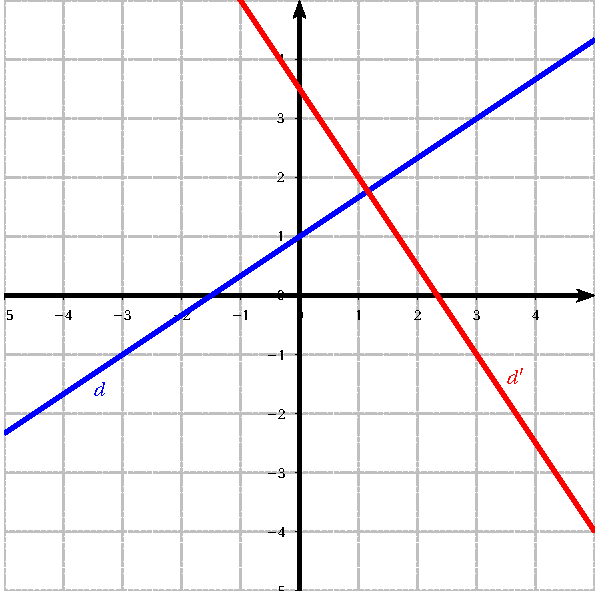
\includegraphics[scale=1]{graphique.pdf}
\end{center}

\begin{enumerate}
\def\labelenumi{\arabic{enumi}.}
\item
  \begin{enumerate}
  \def\labelenumii{(\alph{enumii})}
  \tightlist
  \item
    Déterminer par lecture graphique, un vecteur directeur de la droite
    \(d\) et un point \(A\) appartenant à la droite \(d\).

    \par

    En déduire une équation cartésienne de la droite \(d\).
  \item
    Le point \(B(93;63)\) appartient-il à la droite \(d\) ? Et le point
    \(C(-54;-35)\) ?
  \item
    Que peut-on déduire pour les points \(A\), \(B\) et \(C\) ?
  \end{enumerate}
\item
  \begin{enumerate}
  \def\labelenumii{(\alph{enumii})}
  \tightlist
  \item
    Déterminer l'équation réduite de la droite \(d'\).
  \item
    Montrer que les points \(D(-13;23)\) et \(E(29;-40)\) appartiennent
    à la droite \(d'\).
  \item
    Soit le point \(F(41;-60)\). Les droites \(D\), \(E\) et \(F\)
    sont-ils alignés ? Jusitifer.
  \end{enumerate}
\end{enumerate}

\medskip

\stepcounter{nexo} \underline{\textsc{\textbf{Exercice \arabic{nexo}}}}

Dans chacune des questions suivantes, déterminer si les points \(A\),
\(B\) et \(C\) sont alignés.

\begin{enumerate}
\def\labelenumi{\alph{enumi}.}
\tightlist
\item
  \(A(-6;2)\), \(B(1;1)\) et \(C(4;2)\) ;
\item
  \(A(1;4)\), \(B(-1;-6)\) et \(C(2;9)\).
\end{enumerate}

\medskip

\stepcounter{nexo} \underline{\textsc{\textbf{Exercice \arabic{nexo}}}}

Soient les points \(A(-1;-2)\) et \(B(1;4)\).

\begin{enumerate}
\def\labelenumi{\arabic{enumi}.}
\tightlist
\item
  Déterminer une équation cartésienne de la droite \((AB)\).
\item
  Le point \(C(-3;-9)\) est-il aligné avec les points \(A\) et \(B\) ?
  Qu'en est-il du point \(D(0;1)\).
\item
  Déterminer les réels \(y_F\) et \(x_G\) pour que les points
  \(F(3;y_F)\) et \(G(x_G;-5)\) soient alignés avec \(A\) et \(B\).
\end{enumerate}

\medskip

\newpage

\textbf{Exercice 1}

On considère la suite \((u_n)\) définie pour tout entier naturel \(n\)
par \(u_n = 2n-3\).

\begin{enumerate}
\def\labelenumi{\arabic{enumi})}
\tightlist
\item
  Calculer \(u_0\) et \(u_1\).
\item
  La suite \((u_n)\) est-elle géométrique ? Justifier
\item
  Calculer le cinquième terme de cette suite.
\end{enumerate}

\bigskip

\textbf{Exercice 2}

On considère la suite \((u_n)\) définie pour tout entier naturel \(n\)
par \(u_n = 2n-3\).

\begin{enumerate}
\def\labelenumi{\arabic{enumi}.}
\tightlist
\item
  Calculer

  \begin{enumerate}
  \def\labelenumii{\alph{enumii}.}
  \tightlist
  \item
    la valeur de \(u_0\).
  \item
    la valeur de \(u_1\).
  \end{enumerate}
\item
  La suite \((u_n)\) est-elle géométrique ? Justifier
\item
  Calculer le cinquième terme de cette suite.
\end{enumerate}

\bigskip

\textbf{Exercice 3}

Dans chacune des questions suivantes, déterminer si les points \(A\),
\(B\) et \(C\) sont alignés.

\begin{enumerate}
\def\labelenumi{\alph{enumi}.}
\tightlist
\item
  \(A(-6;2)\), \(B(1;1)\) et \(C(4;2)\) ;
\item
  \(A(1;4)\), \(B(-1;-6)\) et \(C(2;9)\).
\end{enumerate}
